\documentclass{article}
\usepackage[utf8x]{inputenc}
\usepackage{ucs}
\usepackage{amsmath} 
\usepackage{amsfonts}
\usepackage{marvosym}
\usepackage{wasysym}
\usepackage{upgreek}
\usepackage[english,russian]{babel}
\usepackage{graphicx}
\usepackage{float}
\usepackage{textcomp}
\usepackage{hyperref}
\usepackage{geometry}
  \geometry{left=2cm}
  \geometry{right=1.5cm}
  \geometry{top=1cm}
  \geometry{bottom=2cm}
\usepackage{tikz}
\usepackage{ccaption}
\usepackage{multicol}

\hypersetup{
   colorlinks=true,
   citecolor=blue,
   linkcolor=black,
   urlcolor=blue
}

\usepackage{listings}
%\setlength{\columnsep}{1.5cm}
%\setlength{\columnseprule}{0.2pt}

\usepackage[absolute]{textpos}


\usepackage{colortbl,graphicx,tikz}
\definecolor{X}{rgb}{.5,.5,.5}

\renewcommand{\thesubsection}{\arabic{subsection}}

\begin{document}
\pagenumbering{gobble}
\lstset{
  language=C++,                % choose the language of the code
  basicstyle=\linespread{1.1}\ttfamily,
  columns=fixed,
  fontadjust=true,
  basewidth=0.5em,
  keywordstyle=\color{blue}\bfseries,
  commentstyle=\color{gray},
  stringstyle=\ttfamily\color{orange!50!black},
  showstringspaces=false,
  numbersep=5pt,
  numberstyle=\tiny\color{black},
  numberfirstline=true,
  stepnumber=1,                   % the step between two line-numbers.        
  numbersep=10pt,                  % how far the line-numbers are from the code
  backgroundcolor=\color{white},  % choose the background color. You must add \usepackage{color}
  showstringspaces=false,         % underline spaces within strings
  captionpos=b,                   % sets the caption-position to bottom
  breaklines=true,                % sets automatic line breaking
  breakatwhitespace=true,         % sets if automatic breaks should only happen at whitespace
  xleftmargin=.2in,
  extendedchars=\true,
  keepspaces = true,
}
\lstset{literate=%
   *{0}{{{\color{red!20!violet}0}}}1
    {1}{{{\color{red!20!violet}1}}}1
    {2}{{{\color{red!20!violet}2}}}1
    {3}{{{\color{red!20!violet}3}}}1
    {4}{{{\color{red!20!violet}4}}}1
    {5}{{{\color{red!20!violet}5}}}1
    {6}{{{\color{red!20!violet}6}}}1
    {7}{{{\color{red!20!violet}7}}}1
    {8}{{{\color{red!20!violet}8}}}1
    {9}{{{\color{red!20!violet}9}}}1
}
\newcommand\upquote[1]{\textquotesingle#1\textquotesingle}

\renewcommand{\thesubsection}{\arabic{subsection}}
\makeatletter
\def\@seccntformat#1{\@ifundefined{#1@cntformat}%
   {\csname the#1\endcsname\quad}%    default
   {\csname #1@cntformat\endcsname}}% enable individual control
\newcommand\section@cntformat{}     % section level 
\newcommand\subsection@cntformat{Задача \thesubsection.\space} % subsection level
\newcommand\subsubsection@cntformat{\thesubsubsection.\space} % subsubsection level
\makeatother


\makeatletter
\newcount\my@repeat@count
\newcommand{\myrepeat}[2]{%
  \begingroup
  \my@repeat@count=\z@
  \@whilenum\my@repeat@count<#1\do{#2\advance\my@repeat@count\@ne}%
  \endgroup
}
\makeatother

\title{Семинар \#5: Контейнеры STL. Домашнее задание.\vspace{-5ex}}\date{}\maketitle

\subsection{Задача Иосифа Флавия}

\begin{multicols}{2}
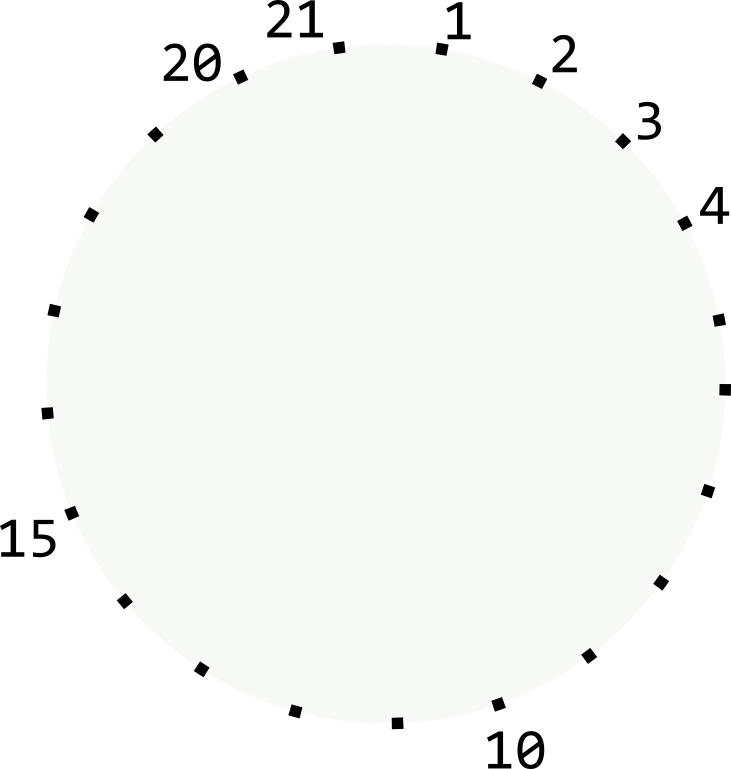
\includegraphics[scale=1]{../images/josephus.png}

По кругу стоит $n$ войнов, начиная с первого война они убивают каждого $m$-го. В каком порядке будут выбывать войны и в каком месте нужно встать, чтобы остаться последним выжившим?\\

Например, если $n = 21$, а $m = 2$, то войны будут выбывать в следующем порядке:
\begin{verbatim}
2 4 6 8 10 12 14 16 18 20 1 5 9 13 17 21 7 15 3 19
\end{verbatim}
В конце останется войн с номером 11.\\

Решите эту задачу, промоделировав ситуацию с помощью контейнера \texttt{std::list}.
\end{multicols}
\begin{center}
\begin{tabular}{ l | l }
 вход & выход \\ \hline
 \texttt{21 2} & \texttt{2 4 6 8 10 12 14 16 18 20 1 5 9 13 17 21 7 15 3 19}\\
 			   & \texttt{11} \\ \hline
 \texttt{7 2} & \texttt{2 4 6 1 5 3}\\
 			   & \texttt{7} \\ \hline
 \texttt{21 6} & \texttt{6 12 18 3 10 17 4 13 21 9 20 11 2 16 14 8 15 1 19 7}\\
 			   & \texttt{5} \\
\end{tabular}
\end{center}


\subsection{Правильная скобочная последовательность}
На вход приходит строка, содержащая некоторою скобочную последовательность. Она может состоять из трёх видов скобок: \texttt{()\{\}[]}. Вам нужно узнать, является ли эта скобочная последовательность правильной. Используйте \texttt{std::stack}.
\begin{center}
\begin{multicols}{2}
\begin{tabular}{ l | l }
 вход & выход \\ \hline
 \texttt{(()())} & \texttt{Yes}  \\ 
 \texttt{)(} &  \texttt{No}\\
 \texttt{[(\{\})]} & \texttt{Yes}  \\ 
 \texttt{)]\}} & \texttt{No}  \\ 
\end{tabular}

\begin{tabular}{ l | l }
 вход & выход \\ \hline
 \texttt{[\}} & \texttt{No}  \\ 
 \texttt{([)]} &  \texttt{No}\\
 \texttt{(\{\}[]([]))[]} & \texttt{Yes}  \\ 
 \texttt{[]} & \texttt{Yes}  \\ 
\end{tabular}
\end{multicols}
\end{center}


\subsection{Верёвка}
На прямой лежит верёвка длиной $n$ метров. Затем её начинают последовательно разрезать, всего сделав $k$ разрезов. Все места разрезов -- целые числа. Найти длину самого длинного куска после каждого разреза. Решение должно иметь вычислительную сложность $O(n \log(n))$. Используйте контейнеры \texttt{std::set} и \texttt{std::multiset}.\\
На вход программе подаются числа $n$ и $k$, а затем $k$ чисел -- места разрезов.
\begin{center}
\begin{tabular}{ l | l }
 вход & выход \\ \hline
 \texttt{20 8} & \texttt{12 10 8 7 6 5 5 4}  \\ 
 \texttt{8 10 15 1 7 4 11 18} &  \\
\end{tabular}
\end{center}

\newpage
\subsection{Количество повторений}
На вход программе приходит $n$ чисел. Некоторые числа могут повторяться. Вам нужно найти уникальныe числа и количество их повторений. Например, если на вход приходят числа \texttt{5 1 5 1 1 1 2 1 5 1}, то среди этих чисел есть 3 уникальных числа: число 1 повторяется 6 раз, число 2 -- 1 раз, а число 5 -- 3 раза. Алгоритм должен работать за $O(n)$ или за $O(n \log(n))$. Используйте контейнер \texttt{std::map}.

\begin{center}
\begin{tabular}{ l | l }
 вход & выход \\ \hline
 \texttt{10} & \texttt{1 2 5}\\
 \texttt{5 1 5 1 1 1 2 1 5 1} & \texttt{6 1 3} \\ \hline
 \texttt{10} & \texttt{2 1000000000}\\
 \texttt{2 2 2 2 2 1000000000 2 2 2 2} & \texttt{9 1} \\
\end{tabular}
\end{center}

\subsection{Поиск пути}
В папке \texttt{wave\_algo\_tests} лежат изображения в формате \texttt{.ppm} (для просмотра изображений в формате \texttt{.ppm} советую использовать программу IrfanView).  Каждая картинка содержит пиксели 4-х разных цветов:
\begin{enumerate}
\item Белые пиксели -- места по которым можно ходить
\item Черные пиксели -- препятствия, то есть места по которым ходить нельзя
\item Зелёный пиксель -- начало пути
\item Красный пиксель -- конец пути
\end{enumerate}
Вам нужно найти кратчайший путь от начала до конца. При этом ходить можно только по пикселям: из одного пикселя можно перейти только в один из восьми соседей.
Кратчайший путь нужно дорисовать на картинке синим цветом и сохранить картинку в новый файл. 
Для работы с изображением используйте класс \texttt{Image}, который находится в папке \texttt{image}.
Кратчайший алгоритм можно найти с помощью волнового алгоритма. При реализации этого алгоритма используйте стандартные контейнеры

\end{document}
